\documentclass{article}

\usepackage{amsmath}
\usepackage{amssymb}
\usepackage{amsthm}
\usepackage{tikz}
\usepackage{listings}
\usepackage{hyperref}
\usepackage[margin=1in]{geometry}
\usepackage{xcolor}

\usetikzlibrary{calc, angles, quotes, decorations.markings}

\definecolor{codebg}{RGB}{245,245,248}
\definecolor{codekw}{RGB}{30,90,170}
\definecolor{codecm}{RGB}{120,120,120}
\definecolor{codest}{RGB}{160,60,60}

\lstset{
  language=JavaScript,
  basicstyle=\ttfamily\footnotesize,
  backgroundcolor=\color{codebg},
  keywordstyle=\color{codekw}\bfseries,
  commentstyle=\color{codecm}\itshape,
  stringstyle=\color{codest},
  showstringspaces=false,
  breaklines=true,
  frame=single,
  framesep=4pt,
  xleftmargin=6pt,
  xrightmargin=6pt,
  numbers=none,
  tabsize=2,
}

\title{Guide 02: Trigonometry for 3D \\ \large web-3d-panel-navigation math curriculum}
\author{}
\date{}

\begin{document}
\maketitle

\section{Why this matters}

In Guide 01 you saw the line \lstinline{Math.acos(fwdDot)} appear in
\texttt{src/camera-transitions.ts} and were told that the dot product of two
unit vectors equals $\cos\theta$. That gave you a vector intuition; this guide
gives you the trig that actually closes the loop. Three places in this codebase
fail without this material:

\begin{itemize}
  \item \texttt{src/zoom-plane-parser.ts:95--97, 215} -- author-supplied
    rotations are in \emph{degrees}; Three.js eats \emph{radians}. The helper
    \lstinline{degreesToRadians} sits at the boundary. Why $\pi/180$?
  \item \texttt{src/projection.ts:175--177} -- the line
    \lstinline{2 * distance * Math.tan(fovRadians / 2)} computes the world-space
    height of the viewport at a plane. That formula is a right-triangle
    statement. We will derive it.
  \item \texttt{src/camera-controller.ts:51--57} -- the same
    $\tan(\theta/2)$ identity, used in reverse: given a desired plane size,
    solve for the camera distance that makes it fill the view.
  \item \texttt{src/camera-transitions.ts:63--71} -- \lstinline{Math.acos} is
    fragile. The codebase clamps its input to $[-1,1]$ first. We will explain
    exactly which floating-point sin a clamp prevents.
\end{itemize}

By the end of this guide, every numeric appearance of
$\sin$, $\cos$, $\tan$, $\arccos$, $\pi$, $180$, or $\theta/2$ in the
project should read like English to you.

\section{Building intuition}

\subsection{The unit circle}

Pick a point on a circle of radius~$1$ centered at the origin. Sweep an angle
$\theta$ counter-clockwise from the positive $x$-axis. The point's
$x$-coordinate is $\cos\theta$ by definition; its $y$-coordinate is
$\sin\theta$. That is the \emph{whole} unit-circle definition.

\begin{center}
\begin{tikzpicture}[scale=2.6]
  \draw[->] (-1.25,0) -- (1.35,0) node[right] {$x$};
  \draw[->] (0,-1.25) -- (0,1.35) node[above] {$y$};
  \draw (0,0) circle (1);

  \coordinate (P) at ({cos(38)},{sin(38)});
  \draw[thick] (0,0) -- (P);
  \filldraw (P) circle (0.8pt);

  \draw[dashed] (P) -- ({cos(38)},0);
  \draw[dashed] (P) -- (0,{sin(38)});

  \draw[->, thick] (0.32,0) arc (0:38:0.32);
  \node at (0.45,0.13) {$\theta$};

  \node[below] at ({cos(38)/2},0) {$\cos\theta$};
  \node[left]  at (0,{sin(38)/2}) {$\sin\theta$};
  \node[above right] at (P) {$(\cos\theta,\,\sin\theta)$};
\end{tikzpicture}
\end{center}

The Pythagorean theorem on the dashed right triangle reads
$\cos^2\theta + \sin^2\theta = 1^2$. That single line (the \emph{Pythagorean
identity}) is the source of half the trig tricks you will ever use.

The third primary function is the slope of the radius vector,
\(
  \tan\theta = \dfrac{\sin\theta}{\cos\theta},
\)
which equals \emph{opposite over adjacent} in the right triangle.

\subsection{Right triangles and ``opposite over adjacent''}

Strip the circle away. A right triangle with one acute angle $\theta$ has three
sides: the side \emph{opposite} $\theta$, the side \emph{adjacent} to $\theta$,
and the hypotenuse. Define

\[
  \sin\theta = \frac{\text{opp}}{\text{hyp}}, \qquad
  \cos\theta = \frac{\text{adj}}{\text{hyp}}, \qquad
  \tan\theta = \frac{\text{opp}}{\text{adj}}.
\]

\begin{center}
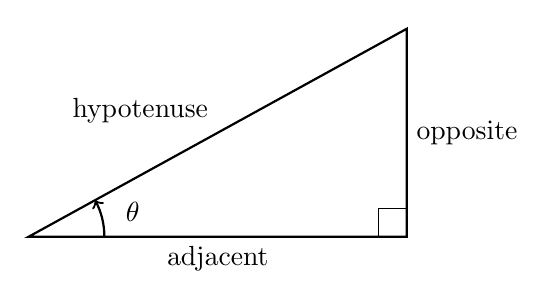
\begin{tikzpicture}[scale=2.4]
  \draw[thick] (0,0) -- (2,0) -- (2,1.1) -- cycle;
  \draw (1.85,0) -- (1.85,0.15) -- (2,0.15);
  \draw[->, thick] (0.4,0) arc (0:28.8:0.4);
  \node at (0.55,0.13) {$\theta$};
  \node[below] at (1, 0)   {adjacent};
  \node[right] at (2, 0.55){opposite};
  \node[above left] at (1, 0.55) {hypotenuse};
\end{tikzpicture}
\end{center}

This picture is what we will redraw as a camera frustum. ``Opposite over
adjacent equals tangent'' is the entire derivation of
\lstinline{2 * distance * Math.tan(fovRadians / 2)}.

\subsection{Why radians, not degrees}

A radian is the angle that subtends an arc of length~$1$ on the unit circle.
The whole circumference is $2\pi$, so a full turn is $2\pi$ radians, half a
turn is $\pi$, a quarter is $\pi/2$. Degrees are a human convention
($360$ per turn, divisible by lots of small numbers). Radians are the
calculus-friendly unit: $\frac{d}{d\theta}\sin\theta = \cos\theta$ is only
true when $\theta$ is in radians. Because every JS \lstinline{Math.sin},
\lstinline{Math.cos}, \lstinline{Math.tan} expects radians, the project does
all internal trig in radians and converts at the data boundary.

\section{The math}

\subsection{Conversion}

A full turn is $360^\circ = 2\pi$ rad, so $1^\circ = \pi/180$ rad. Therefore

\[
  \theta_{\text{rad}} = \theta_{\text{deg}} \cdot \frac{\pi}{180},
  \qquad
  \theta_{\text{deg}} = \theta_{\text{rad}} \cdot \frac{180}{\pi}.
\]

This is exactly what \texttt{zoom-plane-parser.ts} writes:

\begin{lstlisting}
function degreesToRadians(degrees: number): number {
  return (degrees * Math.PI) / 180;
}
\end{lstlisting}

\subsection{The Pythagorean identity}

From the unit-circle picture, the radius is the hypotenuse of the dashed right
triangle, and the legs are $\cos\theta$ and $\sin\theta$. The Pythagorean
theorem gives

\[
  \cos^2\theta + \sin^2\theta = 1.
\]

Two useful corollaries: dividing by $\cos^2\theta$ gives
$1 + \tan^2\theta = \sec^2\theta$, and dividing by $\sin^2\theta$ gives
$\cot^2\theta + 1 = \csc^2\theta$. We will not need those forms here, but they
are why the identity is called \emph{the} Pythagorean identity.

\subsection{Inverse functions, domain, and range}

$\sin$, $\cos$, and $\tan$ are not invertible globally; they repeat. To define
inverses we restrict their domains:

\[
\begin{array}{lll}
  \arcsin : [-1, 1] & \to & [-\pi/2,\, \pi/2], \\[3pt]
  \arccos : [-1, 1] & \to & [0,\, \pi], \\[3pt]
  \arctan : (-\infty, \infty) & \to & (-\pi/2,\, \pi/2).
\end{array}
\]

Notice $\arccos$ outputs angles in $[0, \pi]$. That is exactly the range of
``angle between two unit vectors'', because two vectors are at most
$180^\circ = \pi$ rad apart. That is why the project uses \lstinline{acos}
(not \lstinline{asin}) on the dot product.

\paragraph{Why \lstinline{atan2} exists.} Plain $\arctan$ takes a single ratio
$y/x$ and returns an angle in $(-\pi/2, \pi/2)$, losing the quadrant of the
original $(x,y)$ point. \lstinline{Math.atan2(y, x)} takes both coordinates and
returns an angle in $(-\pi, \pi]$, recovering the quadrant. Use it whenever you
have an actual 2D vector, not just a slope.

\subsection{Numerical safety: why \lstinline{arccos} needs a clamp}

Mathematically, the dot product of two unit vectors is in $[-1, 1]$. Numerically,
floating-point rounding can produce values like $1.0000000002$ or
$-1.0000000007$. \lstinline{Math.acos(1.0000000002)} returns \lstinline{NaN},
which then poisons every downstream computation. The fix is a one-line
defense, and the project uses it verbatim:

\begin{lstlisting}
const fwdDot = THREE.MathUtils.clamp(fromFwd.dot(toFwd), -1, 1);
const fwdAngle = Math.acos(fwdDot);
\end{lstlisting}

This is a canonical pattern. Whenever you feed a dot product, a normalized
component, or any quantity that ``should'' be in $[-1,1]$ into \lstinline{acos}
or \lstinline{asin}, clamp first. Treat it as a reflex.

\subsection{The frustum half-height: $h = d \tan(\theta/2)$}

Now we earn the formula on \texttt{projection.ts:176}.

A perspective camera has a vertical field of view $\theta$: the full angle
subtended, top to bottom, by the visible region. Look at the camera from the
side. A horizontal plane sits at distance $d$ in front of the camera. The
visible region on that plane is a vertical segment centered on the camera's
forward axis. Because $\theta$ is the \emph{full} angle and the segment is
centered, the half-angle is $\theta/2$, and the geometry is a right triangle
with adjacent leg $d$ and opposite leg $h$ (the half-height).

\begin{center}
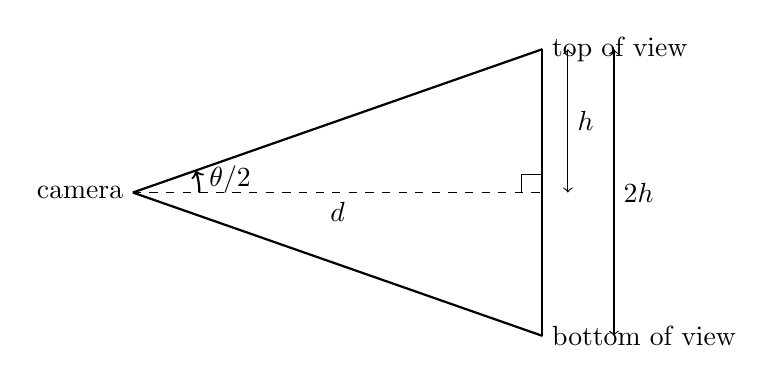
\begin{tikzpicture}[scale=1.3]
  \coordinate (C) at (0,0);
  \coordinate (T) at (4,1.4);
  \coordinate (B) at (4,-1.4);
  \coordinate (M) at (4,0);

  \draw[thick] (C) -- (T);
  \draw[thick] (C) -- (B);
  \draw[dashed] (C) -- (M) node[midway, below] {$d$};
  \draw[thick]  (T) -- (B);

  \draw (3.8,0) -- (3.8,0.18) -- (4,0.18);
  \draw[<->] (4.25,0) -- (4.25,1.4) node[midway, right] {$h$};
  \draw[<->] (4.7,-1.4) -- (4.7,1.4) node[midway, right] {$2h$};

  \draw[->, thick] (0.65,0) arc (0:19.3:0.65);
  \node at (0.95,0.13) {$\theta/2$};

  \node[left] at (C) {camera};
  \node[right] at (T) {top of view};
  \node[right] at (B) {bottom of view};
\end{tikzpicture}
\end{center}

Opposite over adjacent reads
\(
  \tan(\theta/2) = h/d,
\)
so

\[
  h = d \tan(\theta/2), \qquad \text{full height} = 2 d \tan(\theta/2).
\]

That is the \lstinline{viewportHeightAtPlane} line. The horizontal version
multiplies by the aspect ratio; the project does this and we will see it
below, but the full dual-axis aspect-ratio story belongs to Guide 08.

\section{In this codebase}

\subsection{Degrees to radians at the data boundary}

\begin{lstlisting}
// src/zoom-plane-parser.ts (lines 95-97)
function degreesToRadians(degrees: number): number {
  return (degrees * Math.PI) / 180;
}

// src/zoom-plane-parser.ts (line 215)
rotation: parseToThreeTuple(rotationStr, id, 'rotation', degreesToRadians),
\end{lstlisting}

The HTML author writes \lstinline{data-rotation="0,45,0"} in degrees because
that is the unit humans think in. By the time the value reaches Three.js it
must be radians, because every \lstinline{Math.sin}/\lstinline{cos}/\lstinline{tan}
inside Three.js (and inside the rotation matrices we will meet in Guide 04)
expects radians. The conversion happens once, at parse time, and every
downstream consumer can assume radians.

\subsection{Viewport height at a plane}

\begin{lstlisting}
// src/projection.ts (lines 175-177)
const fovRadians = (camera.fov * Math.PI) / 180;
const viewportHeightAtPlane = 2 * distance * Math.tan(fovRadians / 2);
const viewportWidthAtPlane = viewportHeightAtPlane * (viewportWidth / viewportHeight);
\end{lstlisting}

Three.js stores \lstinline{camera.fov} in degrees (one of its few
degrees-flavored fields). Line~175 converts; line~176 is exactly
$2 d \tan(\theta/2)$ from the diagram above; line~177 widens the height by the
aspect ratio because the visible \emph{rectangle} on the plane has the same
aspect ratio as the screen.

\subsection{Distance from desired size: the formula in reverse}

\begin{lstlisting}
// src/camera-controller.ts (lines 51-57)
const fovRadians = (targetFov * Math.PI) / 180;
const halfFovTan = Math.tan(fovRadians / 2);
const fill = this.config.fillPercentage;

const distanceForHeight = (actualHeight / 2) / (halfFovTan * fill);
const distanceForWidth  = (actualWidth  / 2) / (halfFovTan * fill * viewportAspect);
const distance = Math.max(distanceForHeight, distanceForWidth);
\end{lstlisting}

Algebraically, $h = d \tan(\theta/2)$ inverts to $d = h / \tan(\theta/2)$.
Caching $\tan(\theta/2)$ once as \lstinline{halfFovTan} avoids recomputing it.
The \lstinline{fill} factor (e.g. $0.9$) shrinks the target size so the plane
does not touch the screen edges; dividing by it pushes the camera back
proportionally. Taking the \lstinline{Math.max} of the two distances
guarantees neither dimension overflows the viewport. (We will return to the
aspect-ratio split in Guide 08; for now, treat it as: ``solve for height,
solve for width, take whichever needs the camera farther.'')

\subsection{Angle between two orientations, with the safety clamp}

\begin{lstlisting}
// src/camera-transitions.ts (lines 63-71)
// Forward angle
const fromFwd = new THREE.Vector3().subVectors(from.target, from.position).normalize();
const toFwd   = new THREE.Vector3().subVectors(to.target,   to.position  ).normalize();
const fwdDot  = THREE.MathUtils.clamp(fromFwd.dot(toFwd), -1, 1);
const fwdAngle = Math.acos(fwdDot);

// Up angle (captures roll/tilt that forward angle misses)
const upDot   = THREE.MathUtils.clamp(from.up.dot(to.up), -1, 1);
const upAngle = Math.acos(upDot);
\end{lstlisting}

Two unit vectors $\hat{\mathbf{a}}, \hat{\mathbf{b}}$ satisfy
$\hat{\mathbf{a}} \cdot \hat{\mathbf{b}} = \cos\theta$ (Guide 01), so
$\theta = \arccos(\hat{\mathbf{a}} \cdot \hat{\mathbf{b}})$. The clamp exists
because \lstinline{normalize()} is not bit-exact: a vector that is mathematically
unit-length can come back with magnitude $1 + 10^{-16}$, and the dot product
amplifies that. \lstinline{Math.acos(1.0000000001)} is \lstinline{NaN}; the
clamp prevents it.

\section{Worked examples}

\subsection*{Example 1: convert a $45^\circ$ rotation}

A panel declares \lstinline{data-rotation="0,45,0"}. What does
\lstinline{degreesToRadians(45)} return?

\[
  45 \cdot \frac{\pi}{180} = \frac{45\pi}{180} = \frac{\pi}{4} \approx 0.7853981633974483.
\]

That value is what gets stored in \lstinline{plane.rotation[1]} and later
fed to a \lstinline{THREE.Euler}.

\subsection*{Example 2: viewport height at a plane}

The project's default detail FOV is $50^\circ$ and a plane sits $20$ world
units away from the camera. What is the viewport height at the plane?

\[
  \theta = 50^\circ = \frac{50\pi}{180} \approx 0.8727 \text{ rad}.
\]
\[
  \tan(\theta/2) = \tan(25^\circ) \approx 0.4663.
\]
\[
  \text{height} = 2 \cdot 20 \cdot 0.4663 \approx 18.65 \text{ world units}.
\]

If the viewport itself is $1600 \times 900$ pixels (aspect $\approx 1.778$),
the viewport width at the plane is $18.65 \cdot 1.778 \approx 33.16$ world
units. A $1600 \times 900$ plane (in world units) at this distance therefore
\emph{exactly} fits horizontally and overflows vertically by a lot --- which
tells us $20$ is too close for that plane.

\subsection*{Example 3: solve for the camera distance that frames a panel}

Same FOV ($50^\circ$), \lstinline{fillPercentage = 0.9}, plane size
$1600 \times 900$ at \lstinline{scale = 1}, viewport aspect $1.778$. What
distance does \lstinline{calculatePerpendicularState} pick?

\[
  \tan(25^\circ) \approx 0.4663.
\]
\[
  d_{\text{height}} = \frac{900/2}{0.4663 \cdot 0.9}
    = \frac{450}{0.4197} \approx 1072.2,
\]
\[
  d_{\text{width}}  = \frac{1600/2}{0.4663 \cdot 0.9 \cdot 1.778}
    = \frac{800}{0.7462} \approx 1072.1.
\]

The two are essentially equal because $1600/900 \approx 1.778$ matches the
viewport aspect. \lstinline{Math.max} picks the larger; the camera ends up at
$d \approx 1072$ world units. This is a sanity check on the formula: when the
panel and the viewport share an aspect ratio, both axes constrain at the same
distance.

\section{Exercises}

\begin{enumerate}
  \item \textbf{(Routine.)} Convert $30^\circ$, $90^\circ$, $135^\circ$, and
    $-60^\circ$ to radians, in exact form (multiples of $\pi$) and as decimals.

  \item \textbf{(Routine.)} Using the Pythagorean identity, given
    $\sin\theta = 0.6$ with $\theta \in [0, \pi/2]$, find $\cos\theta$ and
    $\tan\theta$ without a calculator.

  \item \textbf{(Conceptual.)} The project uses \lstinline{Math.acos} for the
    angle between two unit vectors but never \lstinline{Math.asin}. State at
    least two reasons why \lstinline{acos} is the natural choice. (Hint: think
    about the dot-product identity, the range of the inverse function, and the
    range of possible angles.)

  \item \textbf{(Conceptual.)} Suppose someone deletes the
    \lstinline{THREE.MathUtils.clamp(...)} call on
    \texttt{camera-transitions.ts:66} and just writes
    \lstinline{Math.acos(fromFwd.dot(toFwd))}. Describe a concrete scenario
    where this code is mathematically correct in exact arithmetic but produces
    \lstinline{NaN} at runtime, and explain what visual symptom \lstinline{NaN}
    would cause downstream.

  \item \textbf{(Project-applied.)} The project's default detail FOV is
    $50^\circ$. If you changed it to $90^\circ$, the camera distance computed
    by \texttt{camera-controller.ts:55--57} would change. By what factor does
    \lstinline{distanceForHeight} change for a fixed plane? (Compute the ratio
    $\tan(25^\circ) / \tan(45^\circ)$.) Does the camera move closer or farther?

  \item \textbf{(Project-applied.)} A plane is $1600$ units wide and $900$
    tall. The viewport is $1600 \times 900$ pixels (aspect $1.778$). At
    detail FOV $50^\circ$ and \lstinline{fillPercentage = 1.0} (no margin),
    what camera distance does \texttt{camera-controller.ts:51--57} pick? Now
    at \lstinline{fillPercentage = 0.5}? State the relationship in one
    sentence.

  \item \textbf{(Extension.)} Derive an algebraic simplification: when the
    plane's aspect ratio equals the viewport's aspect ratio, show that
    \lstinline{distanceForHeight === distanceForWidth} exactly (in exact
    arithmetic). Use the formulas on \texttt{camera-controller.ts:55--56}.

  \item \textbf{(Extension.)} The line
    \lstinline{viewportWidthAtPlane = viewportHeightAtPlane * (viewportWidth/viewportHeight)}
    on \texttt{projection.ts:177} treats the horizontal direction as if it
    obeyed the same $\tan(\theta/2)$ relation as the vertical. Argue why this
    is exact (not approximate) for a standard perspective camera. Hint:
    similar triangles. (Guide 08 will treat this rigorously; here, sketch the
    geometric reason.)
\end{enumerate}

\section{Where to next}

Guide 03 covers \emph{linear interpolation, easing, and smoothstep} -- the
$t$-parameter machinery used at \texttt{camera-transitions.ts:79} where
\lstinline{smoothstep(lowerAngle, upperAngle, totalAngle)} blends between two
transition strategies based on the very angles you computed in this guide.
Guide 04 then takes the radian-valued Euler tuples that
\lstinline{degreesToRadians} produced and turns them into rotation matrices,
making the connection between angle scalars and 3D orientation rigorous.
Slerp (Guide 10) will revisit \lstinline{acos} together with $\sin$ ratios; we
have set up everything it will need.

\appendix
\section*{Appendix: Solutions}
\addcontentsline{toc}{section}{Appendix: Solutions}

\paragraph{Exercise 1.}
\[
  30^\circ = \frac{\pi}{6} \approx 0.5236, \quad
  90^\circ = \frac{\pi}{2} \approx 1.5708,
\]
\[
  135^\circ = \frac{3\pi}{4} \approx 2.3562, \quad
  -60^\circ = -\frac{\pi}{3} \approx -1.0472.
\]

\paragraph{Exercise 2.}
$\cos^2\theta = 1 - 0.36 = 0.64$, and since $\theta \in [0, \pi/2]$ cosine is
non-negative, so $\cos\theta = 0.8$. Then
$\tan\theta = 0.6/0.8 = 0.75$.

\paragraph{Exercise 3.} (i) The Guide 01 identity is
$\hat{\mathbf{a}} \cdot \hat{\mathbf{b}} = \cos\theta$, which inverts directly
with $\arccos$, no extra step. (ii) The angle between two vectors lies in
$[0, \pi]$, and the range of $\arccos$ is exactly $[0, \pi]$. By contrast,
$\arcsin$ outputs $[-\pi/2, \pi/2]$, which excludes obtuse angles -- two
vectors pointing nearly opposite would silently report an acute angle.

\paragraph{Exercise 4.} If \lstinline{from} and \lstinline{to} have identical
forward vectors (e.g. clicking the same panel twice), then mathematically
$\hat{\mathbf{a}} \cdot \hat{\mathbf{a}} = 1$ exactly. Numerically, after two
independent \lstinline{normalize()} calls, the dot can come back as
$1 + \varepsilon$ for some tiny $\varepsilon > 0$. \lstinline{Math.acos} of
anything strictly greater than~$1$ is \lstinline{NaN}.
\lstinline{NaN} then propagates through the angle blend, the smoothstep, and
the position interpolation, and Three.js receives \lstinline{NaN} positions
which it typically renders by either freezing the camera at its last valid
state or producing entirely blank frames. The clamp prevents this for free.

\paragraph{Exercise 5.}
\[
  \tan(25^\circ) \approx 0.4663, \qquad \tan(45^\circ) = 1.
\]
The ratio is $0.4663 / 1 \approx 0.466$. Since
$d_{\text{height}} \propto 1/\tan(\theta/2)$, increasing the FOV from $50^\circ$
to $90^\circ$ shrinks the distance to about $46.6\%$ of its previous value:
the camera moves substantially \emph{closer}. (A wider FOV captures more of the
world at any given distance, so it can sit closer and still frame the panel.)

\paragraph{Exercise 6.} With \lstinline{fillPercentage = 1.0},
\[
  d_{\text{height}} = \frac{450}{0.4663 \cdot 1.0} \approx 965.0,
\]
\[
  d_{\text{width}} = \frac{800}{0.4663 \cdot 1.0 \cdot 1.778} \approx 964.9.
\]
\lstinline{Math.max} returns about $965$. With
\lstinline{fillPercentage = 0.5}, both numerators are unchanged but the
denominators halve, so each distance doubles to about $1930$. Distance is
inversely proportional to \lstinline{fill}: halving the fill doubles the
distance.

\paragraph{Exercise 7.} Let plane width $W$, plane height $H$, with
$W/H = a$ where $a$ is the viewport aspect. Then
\[
  d_{\text{height}} = \frac{H/2}{T \cdot f}, \qquad
  d_{\text{width}}  = \frac{W/2}{T \cdot f \cdot a}
                    = \frac{(aH)/2}{T \cdot f \cdot a}
                    = \frac{H/2}{T \cdot f},
\]
where $T = \tan(\theta/2)$ and $f$ is the fill factor. The two are
algebraically identical, so \lstinline{Math.max} returns either one and the
result is exact.

\paragraph{Exercise 8.} A perspective camera projects through a single point
(its position). Two parallel planes at distances $d_1$ and $d_2$ in front of
that point cut out similar rectangles; the ratio of any horizontal extent to
any vertical extent is preserved across all such planes. In particular the
ratio (full width at distance $d$) to (full height at distance $d$) equals the
ratio at any other distance, including the distance corresponding to the
screen itself, which is the viewport aspect $W_{\text{vp}}/H_{\text{vp}}$.
Hence $\text{width}_d = \text{height}_d \cdot (W_{\text{vp}}/H_{\text{vp}})$
exactly, by similar triangles -- not by approximation. Guide 08 formalizes
this with the projection matrix.

\end{document}
